\section{ACOT Inverse Cotangent Function}

\subsection{Usage}

Computes the inverse cotangent of its argument.  The general
syntax for its use is
\begin{verbatim}
  y = acot(x)
\end{verbatim}
where \verb|x| is an \verb|n|-dimensional array of numerical type.
\subsection{Function Internals}

The \verb|acot| function is computed from the formula
\[
   \cot^{-1}(x) = \tan^{-1}\left(\frac{1}{x}\right)
\]
\subsection{Examples}

Here is a simple plot of the inverse cotangent function
\begin{verbatim}
--> x1 = -2*pi:pi/30:-0.1;
--> x2 = 0.1:pi/30:2*pi;
--> plot(x1,acot(x1),x2,acot(x2)); grid('on');
\end{verbatim}


\centerline{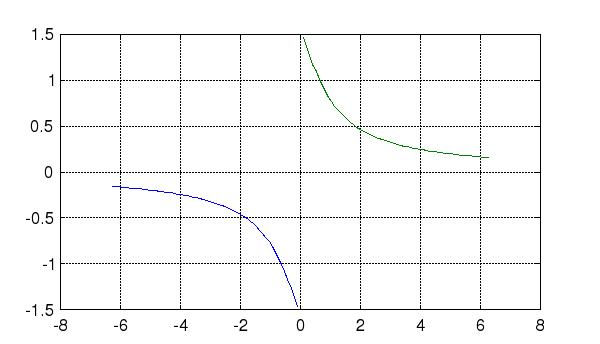
\includegraphics[width=8cm]{acotplot}}

